\chapter{Anhang}


\section{verwendete Programme}

Der Programmcode dieser Arbeit ist unter 
\url{https://github.com/Martin-SF/muography-bachelor}
verfügbar.

Alle Ergebnisse werden mit Python 3.10.4 (\url{https://www.python.org})
mit Hilfe dieser aufgelisteten Bibliotheken erzeugt:
\begin{enumerate}
    \item PROPOSAL 7.3.1 (\url{https://github.com/tudo-astroparticlephysics/PROPOSAL})
    \item EcoMug 1.3.1 (\url{https://github.com/dr4kan/EcoMug})
    \item Numpy 1.21.6 (\url{https://numpy.org/})
    \item pandas 1.4.2 (\url{https://pandas.pydata.org/})
    \item matplotlib 3.5.2 (\url{https://matplotlib.org/})
    \item distributed 2022.5.0 (\url{https://distributed.dask.org/en/stable/})
    \item tqdm 4.64.0 (\url{https://github.com/tqdm/tqdm})
    \item numba 0.55.1 (\url{https://numba.pydata.org/})
    \item pytables 3.7.0 (\url{https://www.pytables.org/})
    \item prettytable 3.2.0 (\url{https://pypi.org/project/prettytable/})
    \item scipy 1.8.0 (\url{https://scipy.org/})
    \item uncertainties 3.1.6 (\url{https://pythonhosted.org/uncertainties/})
\end{enumerate}

%  \marktodo{standort in eigenes figure} 
\section{Schichtverzeichnis}
\label{sec:alle_schichten}
\begin{figure}
    \centering
    % 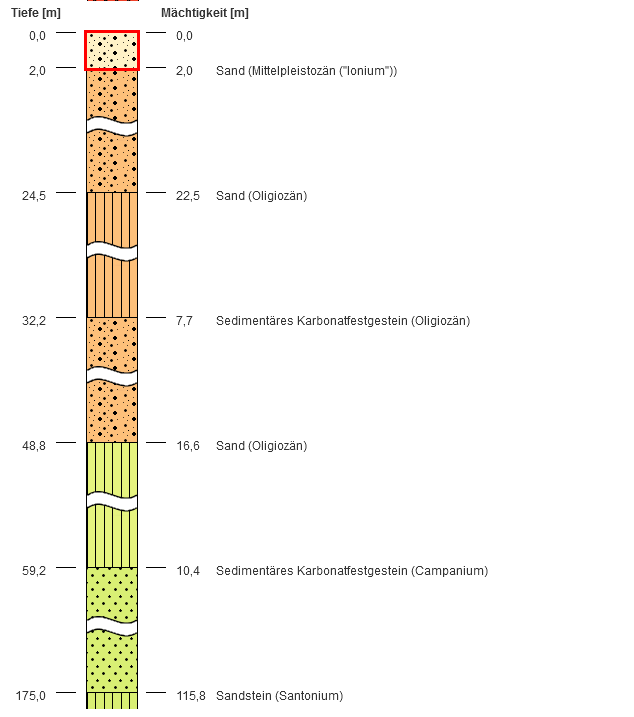
\includegraphics[width=0.49\textwidth]{schichtverzeichnis_1.png}
    % 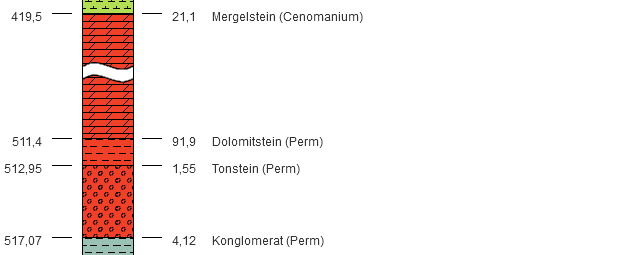
\includegraphics[width=0.49\textwidth]{schichtverzeichnis_3.png}
    % 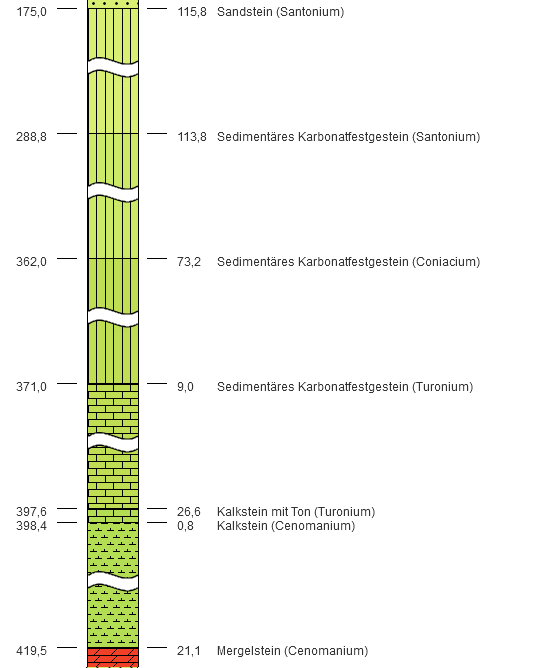
\includegraphics[width=0.49\textwidth]{schichtverzeichnis_2.png}
    % 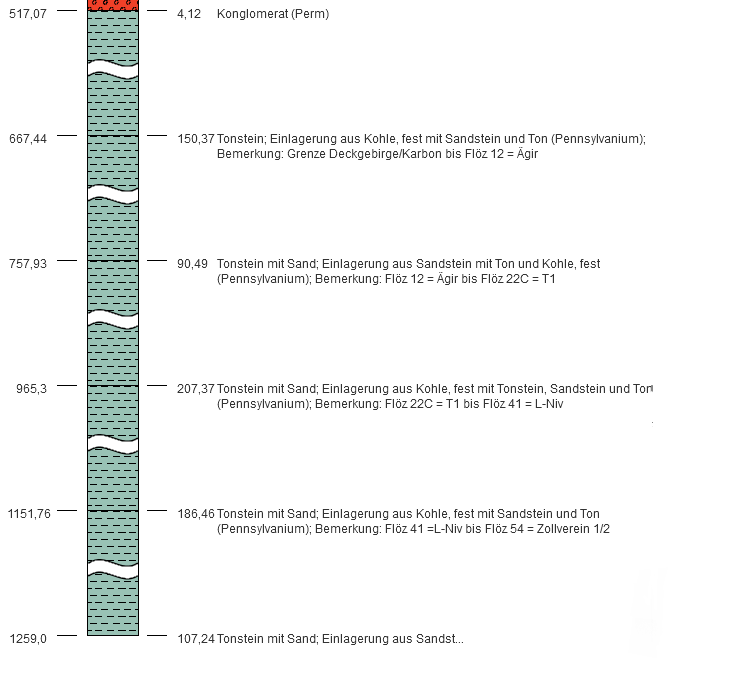
\includegraphics[width=0.49\textwidth]{schichtverzeichnis_4.png}
    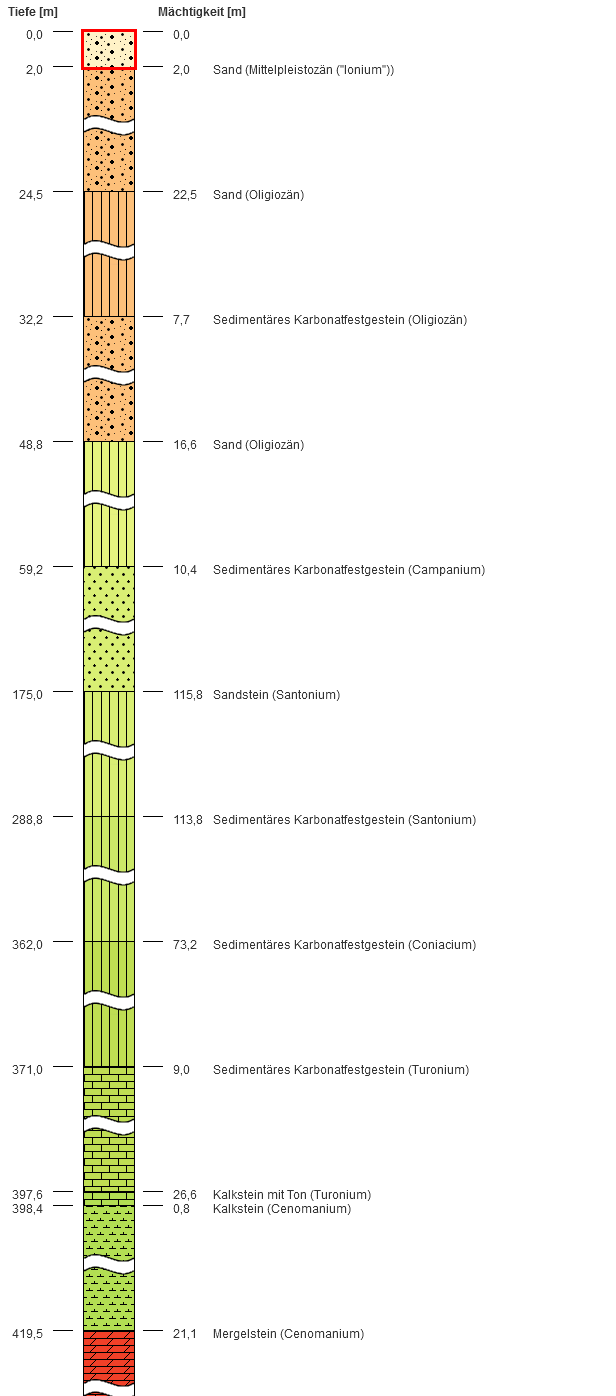
\includegraphics[width=0.49\textwidth]{schichtverzeichnis_10.png}
    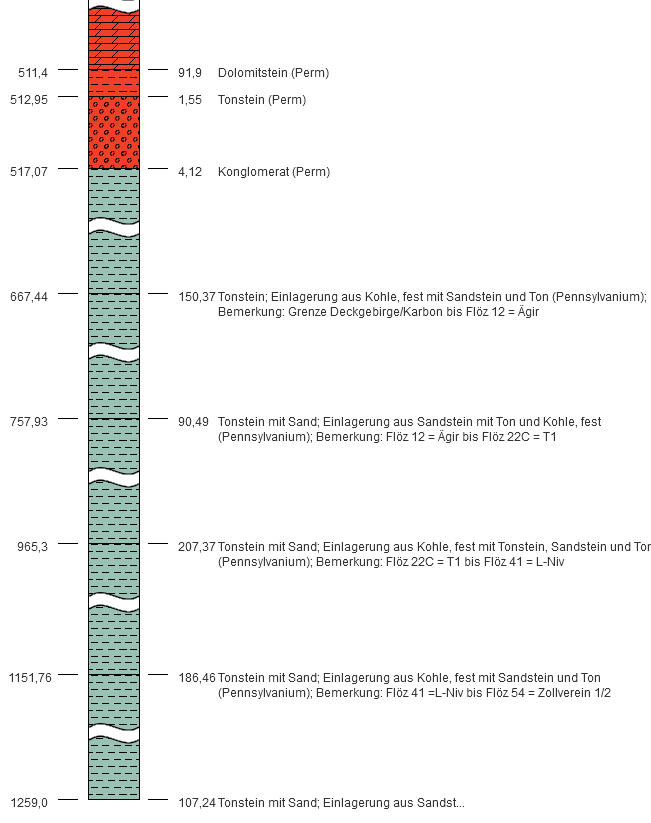
\includegraphics[width=0.49\textwidth]{schichtverzeichnis_11.png}
    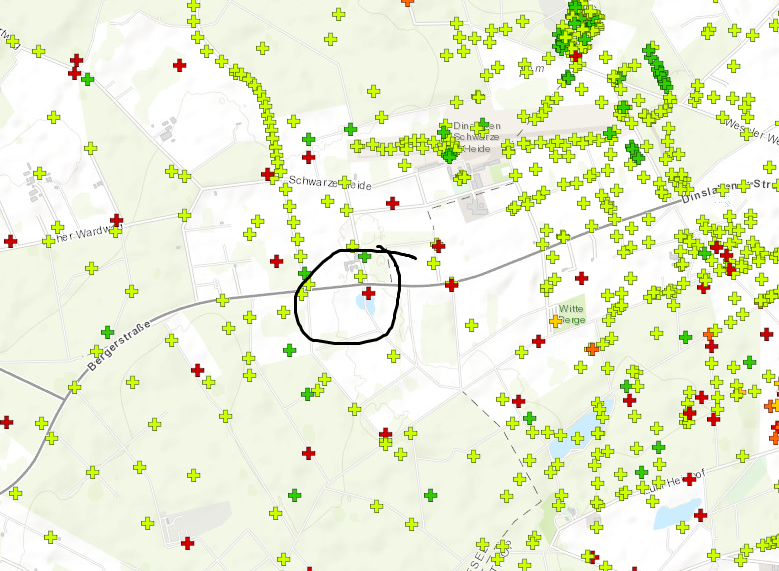
\includegraphics[width=0.49\textwidth]{schichtverzeichnis_location.png}
    \caption{Zu sehen sind die einzelnen Schichten einer Bohrung nahe
     Bottrop. Die erste Zahl steht für die Tiefe des unteren Ende der Schicht in \si[]{m}, die zweite 
    Zahl ist die Dicke der Schicht in \si[]{m}. Der Standort ist im untersten Bild markiert. Zu finden unter 
    \url{boreholemap.bgr.de/mapapps/resources/apps/boreholemap/}. 
    Standort: (\num[]{351221,19} \num[]{5719599,6}) 
    ID: DABO\_65808 (nahe dem Schwarze Heide Airport)}
    \label{fig:Schichtverzeichnis_komplett}
\end{figure}





\section{Konfiguration von EcoMug}
Für EcoMug ist ein Pythoninterface erstellt worden
\footnote{pybind11\url{https://github.com/pybind/pybind11}}. Alle relevanten Funktionen EcoMugs sind nun also auch aus Python benutzbar.
Energieangaben sind in EcoMug immer als Impuls des Teilchens definiert. Zur Vereinheitlichung werden alle
Werte EcoMugs in die Schwerpunktsenergie umgerechnet. 
Mit Dask.distributed wird die Erzeugung der Myonen auf
mehrere Kerne parallelisiert. Jeder Kern zieht einen eigenen zufälligen Seed für EcoMug.

Während erster Testläufe wird festgestellt, dass die in EcoMug standardmäßig verwendete 
Parametrisierung für den Myonenfluss auf Meereshöhe nicht für hohe Energien geeignet ist.


% Es wird aus \cite[]{Alexandrov2017} der Plot aus Abb. \(\)

%  \marktodo{ ändern} 
% Dies ist in Abb. \ref{todo} aus \cite[]{Alexandrov2017} mit EcoMugs Standard
% Parametrisierung erstellt, zu sehen in Abb. \ref{todo}.

% % todo figure fig 4
%  \marktodo{todo} In Abb. \ref{fig:} ist zu sehen wie in Abhängigkeit zu $\cos\theta$ (Zenit Winkel),
% die Energie sinkt.


%  \marktodo{$\theta \leq 30°$ erklären/motivieren.} 
% Es wird zwar EcoMug auf $\theta \leq 30°$ konfiguriert siehe Sektion \ref{sec:pp-config}, 
% dennoch ist selbst für diesen Bereich eine Abweichung zu sehen.
%  \marktodo{andere plots von std vs gaisser wo sich die unterschiede deutlicher zeigen}  

 In Testläufen ergibt sich eine Menge von 
\num{e7} Myonen als geeignetes Mittelmaß zwischen Präzision und 
Laufzeit
Auf dem \textit{phobos} Server des Lehrstuhls benötigt 
EcoMug ca. eine Minute und PROPOSAL ca. \SI[]{30}[]{min} um 10 Mio. Myonen zu generieren bzw. zu propagieren
pro Wassertiefe. Specs: 2x Intel(R) Xeon(R) CPU E5-2680 v3 @ 2.50GHz (je 12 Kerne); 128 GB RAM.

Außerdem ergibt sich, dass Myonen min. über \SI[]{600}[]{GeV} je nach Wasserstand 
brauchen, um den Detektor erreichen zu können.
Bei \SI[]{8}[]{m} Wasserstand haben Myonen mit der geringsten Energie \SI[]{638.9}[]{GeV} (\num[]{1e7} 
simulierte Myonen)
Aufgrund dessen wird in EcoMug die minimale Myonenenergie auf \SI[]{600}[]{GeV} gesetzt.

Ohne diesen Energieschnitt haben die hochenergetischsten Myonen bei \num{e7} erzeugten
ca. \SI[]{200}[]{GeV} wie in Abb. \ref{fig:minenergieplot} zu sehen.

% oberhalb von \SI[]{800}[]{GeV}, nun sind es mit der Anpassung einstellige Prozentbereiche.
%  \marktodo{kleiner machen, mit anderem plot vereinen} 

\begin{figure}[h]
    \centering
    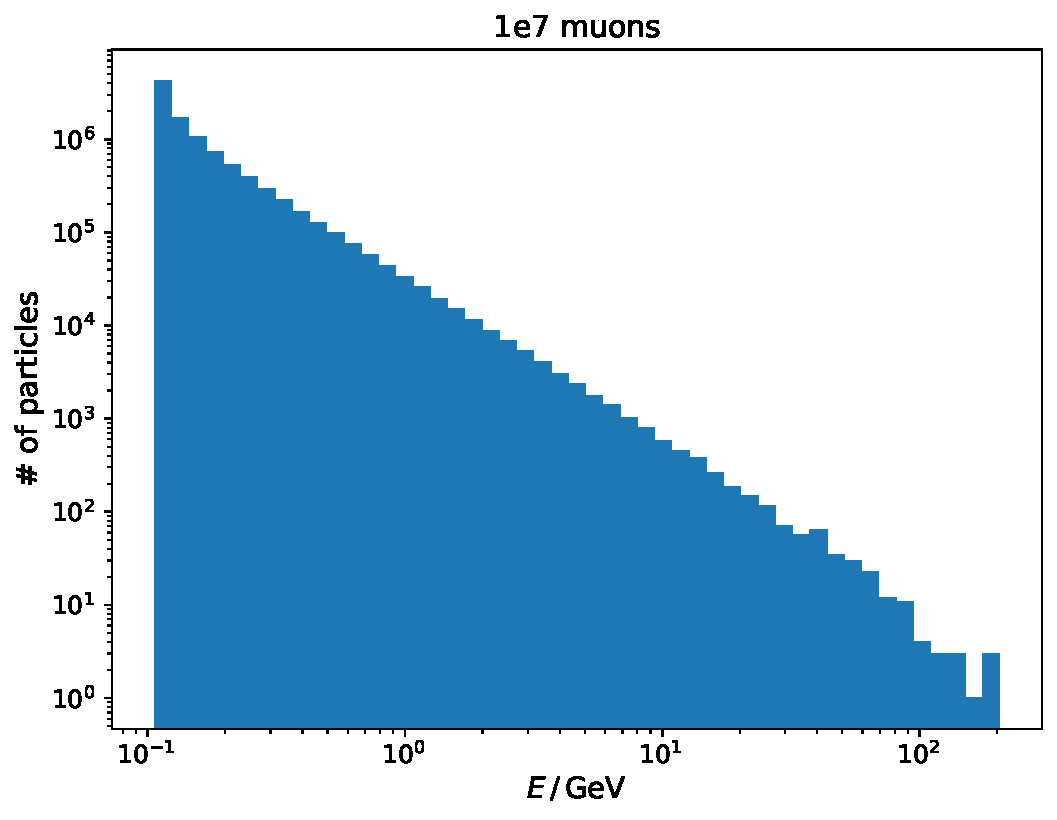
\includegraphics[width=0.7\textwidth]{1e7 muons.pdf}
    \caption{10 Mio. Myonen mit EcoMug (Gaisser) ohne Energieschnitt erzeugt.
    Die maximale Energie liegt lediglich bei ca. \SI[]{200}[]{GeV}. }
    \label{fig:minenergieplot}
\end{figure}

In Testläufen mit \num{e7} Myonen ergibt sich wie in Abb. \ref{fig:ecomugplot} zu sehen,
dass die hochenergetischsten Myonen unter \SI[]{100}[]{TeV} bleiben.

Deshalb wird die maximale Myonenenergie in EcoMug auf \SI[]{200}[]{TeV} gesetzt. 
\footnote{Der Grund dafür ist, dass EcoMugs Laufzeit mit der Breite des Energiebereichs skaliert. 
Es sollte also ein Energiemaximum leicht oberhalb des maximalen $E_\mu$ gewählt werden.}  

% restliche Konfiguration#
Des Weiteren wird die Generationsfläche auf einen Punkt vereinfacht (siehe Kap. \ref{sec:pp-config}),
d.h. jedes Myon hat als Start Position
(0,0,0)\footnote{
    Zur Vermeidung unnötiger Zyklen wird im gesamten Programmcode
    angenommen das die Myonen bei (0,0,0) starten.}
Im Abschnitt \ref{sec:pp-config}
findet sich die Begründung.


\section{Konfiguration von PROPOSAL}

Da das erstellte Bodenmodell eindimensional ist und die verwendete Gaisser-Parametrisierung
(siehe Kap. \ref{sec:myonenfluss}) $\theta < 70°$ vorschreibt, da es die Erdkrümmung
vernachlässigt, wird sich folgende Näherung überlegt:
Es wird die Emissionsfläche der Myonen mit dem, in der Größenordnung des Experiments 
punktförmigen Detektor, vertauscht.
Diese Näherung garantiert das jedes Myon, soweit es genug Energie besitzt, den Detektor trifft.
% Dies ist die Optimierung mit der höchsten Laufzeit Verbesserung in dieser Arbeit.

Zu den in Kap. \ref{sec:bodenmodell} beschriebenen Schichten wird der PROPOSAL 
Konfiguration noch eine Detektorschicht hinzugefügt und eine \textit{hierarchy}
von 20 gegeben. Die \textit{hierarchy}-Bedingung wird dazu benutzt zu definieren, 
wann PROPOSAL mit der Propagation stoppen soll.
Diese Schicht repräsentiert ohne die am 
Anfang des Kapitels beschriebene Näherung anschaulich die Fläche der Myonen aus der Atmosphäre,
welche den Detektor treffen. 

% Zur Auswahl des Energy-Cuts und der Vielfachstreuung werden Tests gemacht,
% dessen Ergebnisse in Abb. \ref{fig:cut_scat_tests} zu sehen sind.

% \marktodo{fig} 
% \begin{figure}[h]
%     \centering
%     \includegraphics{}
%     \caption{Zu sehen die Anzahl an Myonen, die an einem Detektor in \SI[]{1205}[]{m}}
%     angekommen sind, in Abhängigkeit zu $v_\mathrm{cut}$ und verschiedene Vielfachstreuungen.}
%     \label{fig:cut_scat_tests}
% \end{figure}

Für die Berechnung der Ergebnisse wird folgende Konfiguration verwendet:
\begin{align}
    v_\mathrm{cut} = 0.001  \;\; \mathrm{und} \;\; \mathrm{multiplescattering} = \mathrm{Highland}
\end{align}

% Zur finalen Propagation lädt PROPOSAL die von EcoMug erzeugten Myonen aus einer HDF5-Datei.
% Es wird Teilchenart, Energie und Richtung ausgelesen. Die Position wird für jedes Teilchen statisch
% auf (0,0,0) gesetzt.
% Nun propagiert PROPOSAL bis zum Zerfall des Teilchens oder bis es den Detektor erreicht hat.
% Dazu wird aus dem \textit{track}-Objekt welches PROPOSAL als Ergebnis ausgibt, 
% die $z$-Koordinate ausgelesen verglichen mit der des Detektor-Sektors.
% Hat das Myon den Detektor erreicht, wird 
% der  \marktodo{output } in eine HDF5-Datei gespeichert. Der Name der Datei enthält außerdem
%  die Anzahl an Myonen die insgesamt propagiert wurden.

 Zur weiteren Optimierung der Laufzeit wird wieder mit Dask.distributed 
 eine Parallelisierung auf mehreren Kernen ermöglicht. Da PROPOSAL einen standardmäßigen
 Seed setzt erzeugt sich jeder Kern einen neuen zufälligen Seed.